%%%%%%%%%%%%%%%%%%%%%%%%%%%%%%%%%%%%%%%%%
% Lachaise Assignment
% LaTeX Template
% Version 1.0 (26/6/2018)
%
% This template originates from:
% http://www.LaTeXTemplates.com
%
% Authors:
% Marion Lachaise & François Févotte
% Vel (vel@LaTeXTemplates.com)
%
% License:
% CC BY-NC-SA 3.0 (http://creativecommons.org/licenses/by-nc-sa/3.0/)
% 
%%%%%%%%%%%%%%%%%%%%%%%%%%%%%%%%%%%%%%%%%

%----------------------------------------------------------------------------------------
%	PACKAGES AND OTHER DOCUMENT CONFIGURATIONS
%----------------------------------------------------------------------------------------

\documentclass{article}

%%%%%%%%%%%%%%%%%%%%%%%%%%%%%%%%%%%%%%%%%
% Lachaise Assignment
% Structure Specification File
% Version 1.0 (26/6/2018)
%
% This template originates from:
% http://www.LaTeXTemplates.com
%
% Authors:
% Marion Lachaise & François Févotte
% Vel (vel@LaTeXTemplates.com)
%
% License:
% CC BY-NC-SA 3.0 (http://creativecommons.org/licenses/by-nc-sa/3.0/)
% 
%%%%%%%%%%%%%%%%%%%%%%%%%%%%%%%%%%%%%%%%%

%----------------------------------------------------------------------------------------
%	PACKAGES AND OTHER DOCUMENT CONFIGURATIONS
%----------------------------------------------------------------------------------------

\usepackage{amsmath,amsfonts,stmaryrd,amssymb} % Math packages
\newcommand{\Lagr}{\mathcal{L}}

\usepackage{enumerate} % Custom item numbers for enumerations

\usepackage[ruled]{algorithm2e} % Algorithms

\usepackage[framemethod=tikz]{mdframed} % Allows defining custom boxed/framed environments

\usepackage{titlesec}

\usepackage{listings} % File listings, with syntax highlighting
\lstset{
	basicstyle=\ttfamily, % Typeset listings in monospace font
}

\usepackage{physics} % Физические обозначения

\usepackage{indentfirst} % Красная строка в первом предложении

\usepackage{appendix} % Приложения

%----------------------------------------------------------------------------------------
%	DOCUMENT MARGINS
%----------------------------------------------------------------------------------------

\usepackage{geometry} % Required for adjusting page dimensions and margins

\geometry{
	paper=a4paper, % Paper size, change to letterpaper for US letter size
	top=2.0cm, % Top margin
	bottom=2.0cm, % Bottom margin
	left=2.0cm, % Left margin
	right=1.5cm, % Right margin
	headheight=14pt, % Header height
	%footskip=1.5cm, % Space from the bottom margin to the baseline of the footer
	%headsep=0.5cm, % Space from the top margin to the baseline of the header
	%showframe, % Uncomment to show how the type block is set on the page
}

%----------------------------------------------------------------------------------------
%	FONTS
%----------------------------------------------------------------------------------------

%\usepackage[utf8]{inputenc} % Required for inputting international characters
%\usepackage[T1]{fontenc} % Output font encoding for international characters
\usepackage[T1,T2A]{fontenc}
\usepackage[utf8]{inputenc}
\usepackage[english,russian]{babel}

\usepackage{XCharter} % Use the XCharter fonts

%----------------------------------------------------------------------------------------
%	COMMAND LINE ENVIRONMENT
%----------------------------------------------------------------------------------------

% Usage:
% \begin{commandline}
%	\begin{verbatim}
%		$ ls
%		
%		Applications	Desktop	...
%	\end{verbatim}
% \end{commandline}

\mdfdefinestyle{commandline}{
	leftmargin=10pt,
	rightmargin=10pt,
	innerleftmargin=15pt,
	middlelinecolor=black!50!white,
	middlelinewidth=2pt,
	frametitlerule=false,
	backgroundcolor=black!5!white,
	frametitle={Command Line},
	frametitlefont={\normalfont\sffamily\color{white}\hspace{-1em}},
	frametitlebackgroundcolor=black!50!white,
	nobreak,
}

% Define a custom environment for command-line snapshots
\newenvironment{commandline}{
	\medskip
	\begin{mdframed}[style=commandline]
}{
	\end{mdframed}
	\medskip
}

%----------------------------------------------------------------------------------------
%	FILE CONTENTS ENVIRONMENT
%----------------------------------------------------------------------------------------

% Usage:
% \begin{file}[optional filename, defaults to "File"]
%	File contents, for example, with a listings environment
% \end{file}

\mdfdefinestyle{file}{
	innertopmargin=1.6\baselineskip,
	innerbottommargin=0.8\baselineskip,
	topline=false, bottomline=false,
	leftline=false, rightline=false,
	leftmargin=2cm,
	rightmargin=2cm,
	singleextra={%
		\draw[fill=black!10!white](P)++(0,-1.2em)rectangle(P-|O);
		\node[anchor=north west]
		at(P-|O){\ttfamily\mdfilename};
		%
		\def\l{3em}
		\draw(O-|P)++(-\l,0)--++(\l,\l)--(P)--(P-|O)--(O)--cycle;
		\draw(O-|P)++(-\l,0)--++(0,\l)--++(\l,0);
	},
	nobreak,
}

% Define a custom environment for file contents
\newenvironment{file}[1][File]{ % Set the default filename to "File"
	\medskip
	\newcommand{\mdfilename}{#1}
	\begin{mdframed}[style=file]
}{
	\end{mdframed}
	\medskip
}

%----------------------------------------------------------------------------------------
%	NUMBERED QUESTIONS ENVIRONMENT
%----------------------------------------------------------------------------------------

% Usage:
% \begin{question}[optional title]
%	Question contents
% \end{question}

\mdfdefinestyle{question}{
	innertopmargin=1.2\baselineskip,
	innerbottommargin=0.8\baselineskip,
	roundcorner=5pt,
	nobreak,
	singleextra={%
		\draw(P-|O)node[xshift=1em,anchor=west,fill=white,draw,rounded corners=5pt]{%
		Вопрос \theQuestion\questionTitle};
	},
}

\newcounter{Question} % Stores the current question number that gets iterated with each new question

% Define a custom environment for numbered questions
\newenvironment{question}[1][\unskip]{
	\bigskip
	\stepcounter{Question}
	\newcommand{\questionTitle}{~#1}
	\begin{mdframed}[style=question]
}{
	\end{mdframed}
	\medskip
}

%----------------------------------------------------------------------------------------
%	WARNING TEXT ENVIRONMENT
%----------------------------------------------------------------------------------------

% Usage:
% \begin{warn}[optional title, defaults to "Warning:"]
%	Contents
% \end{warn}

\mdfdefinestyle{warning}{
	topline=false, bottomline=false,
	leftline=false, rightline=false,
	nobreak,
	singleextra={%
		\draw(P-|O)++(-0.5em,0)node(tmp1){};
		\draw(P-|O)++(0.5em,0)node(tmp2){};
		\fill[black,rotate around={45:(P-|O)}](tmp1)rectangle(tmp2);
		\node at(P-|O){\color{white}\scriptsize\bf !};
		\draw[very thick](P-|O)++(0,-1em)--(O);%--(O-|P);
	}
}

% Define a custom environment for warning text
\newenvironment{warn}[1][Warning:]{ % Set the default warning to "Warning:"
	\medskip
	\begin{mdframed}[style=warning]
		\noindent{\textbf{#1}}
}{
	\end{mdframed}
}

%----------------------------------------------------------------------------------------
%	INFORMATION ENVIRONMENT
%----------------------------------------------------------------------------------------

% Usage:
% \begin{info}[optional title, defaults to "Info:"]
% 	contents
% 	\end{info}

\mdfdefinestyle{info}{%
	topline=false, bottomline=false,
	leftline=false, rightline=false,
	nobreak,
	singleextra={%
		\fill[black](P-|O)circle[radius=0.4em];
		\node at(P-|O){\color{white}\scriptsize\bf i};
		\draw[very thick](P-|O)++(0,-0.8em)--(O);%--(O-|P);
	}
}

% Define a custom environment for information
\newenvironment{info}[1][Информация:]{ % Set the default title to "Info:"
	\medskip
	\begin{mdframed}[style=info]
		\noindent{\textbf{#1}}
}{
	\end{mdframed}
}

%----------------------------------------------------------------------------------------
%	IMAGES
%----------------------------------------------------------------------------------------

\usepackage{graphicx}
\graphicspath{{images/}}
\DeclareGraphicsExtensions{.pdf,.png,.jpg} % Include the file specifying the document structure and custom commands

%----------------------------------------------------------------------------------------
%	ASSIGNMENT INFORMATION
%----------------------------------------------------------------------------------------

\title{Метод Ритца (Рэлея-Ритца) \#2} % Title of the assignment

\author{Николай Животенко\\ \texttt{niko.zvt@gmail.com}} % Author name and email address

\date{МГТУ им. Н. Э. Баумана --- \today} % University, school and/or department name(s) and a date

%----------------------------------------------------------------------------------------

\begin{document}

\maketitle % Print the title

%----------------------------------------------------------------------------------------
%	Введение
%----------------------------------------------------------------------------------------

\section*{Введение} % Unnumbered section

\begin{info} % Information block
	Вариационное исчисление – математическая дисциплина, посвящённая отысканию экстремальных (наибольших и наименьших) значений функционалов – переменных величин, зависящих от выбора одной или нескольких функций. Вариационное исчисление является естественным развитием той главы математического анализа, которая посвящена задаче отыскания экстремумов функций. Возникновение и развитие вариационного исчисления тесно связано с задачами механики, физики и других технических наук.
\end{info}

Ещё в античные времена появились первые вариационные проблемы, относящиеся к категории изопериметрических задач – например, задача Дидоны. Первый вариационный принцип сформулировал Герон Александрийский для траекторий отражённых световых лучей в работе «Катоптрика» (I в. н.э.). В средневековой Европе изопериметрическими задачами занимались И. Сакробоско (XIII в.) и Т. Брадвардин (XIV в.). После разработки анализа появились новые типы вариационных задач, в основном механического характера. Ньютон в «Математических началах натуральной философии» (1687 г.) решает задачу: найти форму тела вращения, обеспечивающую наименьшее сопротивление при движении в газе или жидкости при заданных размерах. Важной исторической задачей, давшей толчок к развитию современного варианта вариационного исчисления, стала задача о брахистохроне (1696 г.). Её быстрое решение сразу несколькими математиками показало огромные возможности новых методов. Среди других задач стоит отметить определение формы цепной линии, то есть формы равновесия тяжёлой однородной нити (1690 г.). Общих методов решения вариационных задач в этот период ещё не существовало, каждая задача решалась с помощью остроумных и не всегда безупречных геометрических рассуждений.

Решающий вклад в развитие вариационного исчисления внесли Леонард Эйлер и Жозеф Лагранж. Эйлеру принадлежит первое систематическое изложение вариационного исчисления и сам термин (1766 г.). Лагранж независимо получил многие основополагающие результаты и ввёл понятие вариации (с 1755 г.). На этом этапе были выведены уравнения Эйлера – Лагранжа.

Методы вариационного исчисления широко применяются в различных областях математики. Например, в дифференциальной геометрии с их помощью ищут геодезические линии и минимальные поверхности. В физике вариационный метод – одно из мощнейших орудий получения уравнений движения, как для дискретных, так и для распределённых систем, в том числе и для физических полей. Методы вариационного исчисления применимы и в статике.

Выделяют два основных типа методов решения вариационных задач. К первому типу относятся методы, сводящие исходную задачу к решению дифференциальных уравнений. Альтернативой являются так называемые прямые методы. Эти методы тем или иным способом решают исходную задачу по поиску функции в заданном классе, которая доставляла бы экстремальное значение заданному функционалу. Один из самых популярных методов этого класса — метод Ритца (также называемый методом Рэлея-Ритца).

%----------------------------------------------------------------------------------------
%	ГЛАВА 1
%----------------------------------------------------------------------------------------

\newpage

\section{Вариационное исчисление}

\subsection{Понятие функционала}

В курсе высшей математики вводилось понятие функции. Если некоторому числу $x$ из области $D$ ставится в соответствие по определённому правилу или закону число $y$, то говорят, что задана функция $y=f(x)$. Область $D$ называют областью определения функции $f(x)$.

Если же функции $f(x)$ ставится в соответствие по определённому правилу или закону число $J$, то говорят, что задан функционал $J = \Phi[f(x)]$ или 
$J = \Phi[y]$. Примером функционала может быть определённый интеграл от функции $f(x)$ или от некоторого выражения, зависящего от $f(x)$,

\begin{displaymath}
	\Phi[y] = \int_{a}^{b} f(x) \; dx,
\end{displaymath}

\begin{displaymath}
	\Phi[y] = \int_{a}^{b} [f''(x) + p(x)f'(x) + q(x)f(x)] \;  dx.
\end{displaymath}

Если теперь функции $u = f(x, y)$ ставится в соответствие по определённому правилу или закону вновь функция $z = g(u)$, то говорят, что задан оператор $z = L(u)$ или $z = Lu$. Примерами дифференциальных операторов могут служить:

\begin{displaymath}
	Lu = u'' + p(x,y)u' + q(x,y)u,
\end{displaymath}

\begin{displaymath}
    Lu = \frac{\partial^2 u}{\partial x^2} + \frac{\partial^2 u}{\partial y^2}.
\end{displaymath}

Дадим более строгое определение функционала. Пусть $A$ – множество элементов произвольной природы, и пусть каждому элементу $u \in A$ приведено в соответствие одно и только одно число $J = \Phi[u]$. В этом случае говорят, что на множестве $A$ задан функционал $\Phi[u]$. Множество $A$ называется областью определения функционала $\Phi[u]$ и обозначается через $D(J)$; число $J$ называется значением функционала $\Phi[u]$ на элементе $u$. Функционал $\Phi[u]$ называется вещественным, если все его значения вещественны. Функционал $\Phi[u]$ называется линейным, если его область определения есть линейное множество и если

\begin{displaymath}
    \Phi[\alpha u + \beta v] = \alpha \cdot \Phi[u] + \beta \cdot \Phi[v].
\end{displaymath}

%------------------------------------------------

\subsection{Задачи, приводящие к экстремуму функционала}

Зарождение вариационного исчисления относят обычно к 1696 году, когда И. Бернулли поставил так называемую задачу о брахистохроне: определить форму кривой, лежащей в вертикальной плоскости, по которой тяжёлая материальная точка, двигаясь под действием только одной силы тяжести и не имеющая начальной скорости, перейдёт из верхнего положения $A$ в нижнее положение $B$ за минимум времени, рисунок \ref{img_brachistochrone}. Эта задача сводится к отысканию исходной функции $y = f(x)$ – брахистохроны.

\begin{figure}[h!]
\center{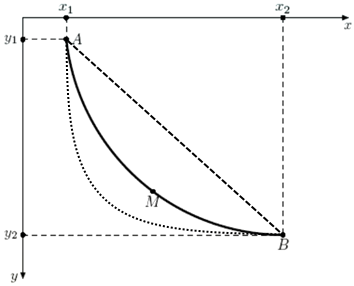
\includegraphics[height=4cm]{images/img_001.png}}
\caption{Задача о брахистохроне}
\label{img_brachistochrone}
\end{figure}

Пусть уравнение кривой $AB$ есть $y = f(x)$. Рассмотрим некоторый момент времени $t$, и пусть в этот момент движущаяся точка находится на расстоянии $y$ от оси $x$. Направим ось ординат вниз и сопоставим начальной точке нулевое значение ординаты. Из закона сохранения энергии для материальной точки имеем

\begin{displaymath}
    \frac{m\upsilon^2}{2} = mgy.
\end{displaymath}

Тогда $\upsilon = \sqrt{2gy}$ , где $\upsilon$ – скорость движущейся точки, $g$ – ускорение свободного падения, a $y$ - ордината точки. В то же время:

\begin{displaymath}
    \upsilon = \frac{dS}{dt} = \sqrt{1 + (y')^2} \frac{dx}{dt},
\end{displaymath}

\noindent отсюда следует, что

\begin{displaymath}
    dt = \sqrt{\frac{1 + (y')^2}{2gy}}dx,
\end{displaymath}

\noindent Обозначим через $T$ время, в течение которого материальная точка достигает точки $B$. Интегрируя, находим

\begin{displaymath}
    T = \frac{1}{\sqrt{2g}} \int_{A}^{B} \sqrt{\frac{1 + (y')^2}{y}} \; dx.
\end{displaymath}

\noindent Задача сводится к следующему: надо найти функцию $y = f(x)$, удовлетворяющую условию $f(A) = 0$, $f(B) = C$ и сообщающую интегралу наименьшее значение. Условия означают, что искомая кривая должна проходить через заданные точки $A$ и $B$. Такого типа условия принято называть граничными, или краевыми, так как они относятся к концам промежутка, на котором должна быть определена искомая функция.

\begin{info}
	Данная задача относится к ветви математического анализа, называемой вариационным исчислением. Примером применения кривой в виде брахистохроны служит образующая цилиндрических поверхностей, используемых на детских площадках, в аттракционах для спуска с возвышения, на трамплинах.
\end{info}

%------------------------------------------------

\subsection{Первая вариация функционала}

Задача вариационного исчисления состоит в следующем: дан функционал $\Phi[u]$ с областью определения $D(\Phi[u])$; требуется найти элемент $u_{0} \in D(\Phi[u])$, сообщающий функционалу либо минимальное значение, либо максимальное. Задача о максимуме функционала $\Phi[u]$ тождественна с задачей о минимуме функционала $- \Phi[u]$.

Будем рассматривать функционал $\Phi[u]$. Возьмём произвольный элемент $u \in D(\Phi[u])$ и произвольный элемент $\eta \in D(\Phi[u]) $. Обозначим через $\alpha$ произвольное вещественное число. Нетрудно видеть, что элемент $ u + \alpha \eta \in D(\Phi[u])$. Составим выражение $\Phi[u + \alpha \eta]$. Данное выражение есть непрерывно дифференцируемая функция от $\alpha$. Вычислим её производную и возьмём значение этой производной при $\alpha = 0$:

\begin{displaymath}
    \frac{d\Phi[u + \alpha \eta]}{d\alpha}.
\end{displaymath}

\noindent В результате получим число, которое можно рассматривать как значение функционала, зависящего от двух элементов $u$ и $\eta$. Функционал

\begin{displaymath}
    \frac{d\Phi[u + \alpha \eta]}{d\alpha} \cdot \alpha
\end{displaymath}

\noindent называется первой вариацией функционала $\Phi[u]$ на элементе $u$ и обозначается символом $\delta \Phi[u, \eta]$:

\begin{displaymath}
     \delta \Phi[u, \eta] = \frac{d\Phi[u + \alpha \eta]}{d\alpha} \cdot \alpha.
\end{displaymath}

\noindent При этом разность двух функций $u_{1} \in D(\Phi[u])$ и $u_{2} \in D(\Phi[u])$ называют вариацией функции $u$ и обозначают $\delta u = u_{1}(x) - u_{2}(x)$.

%------------------------------------------------

\subsection{Необходимое условие минимума функционала}\label{sub_section_minimum_conditions}

Пусть функционал $\Phi[u]$ достигает на некотором элементе $u_{0}$ относительного минимума. Возьмём произвольный элемент $\eta \in D(\Phi[u])$ и произвольное вещественное число $\alpha$. По определению относительного минимума при достаточно малых значениях $\alpha$

\begin{displaymath}
     d\Phi[u_{0} + \alpha\eta] \geq d\Phi[u_{0}].
\end{displaymath}

\noindent Это неравенство означает, что функция одной вещественной переменной $\alpha$, равная $d\Phi[u_{0} + \alpha\eta]$, имеет при $\alpha = 0$ относительный минимум. Но тогда необходимо, чтобы  $\delta \Phi[u_{0}, \eta] = 0$.

\begin{warn}[Важно!]
	Если функционал в некоторой точке достигает минимума, то в этой точке первая вариация функционала равна нулю. В этом заключается необходимое условие экстремума функционала.
\end{warn}

%------------------------------------------------

\subsection{Уравнение Эйлера. Связь между вариационной и краевой задачами}

\begin{warn}[Базовая версия леммы Лагранжа.]
	Если непрерывная функция $f(x)$ на открытом интервале $(a, b)$ удовлетворяет равенству
	
\begin{displaymath}
	\int_{a}^{b} f(x) \cdot h(x) \cdot dx = 0
\end{displaymath}

\noindent для всех финитных гладких функций $h(x)$ на $(a, b)$, тогда $f(x)$ является тождественным нулём.
\end{warn}

Мы хотим найти такую функцию $u = f(x)$, которая удовлетворяет граничным условиям $u(a) = A$, $u(b) = B$ и доставляет экстремум функционалу

\begin{displaymath}
	\Phi[u] = \int_{a}^{b} L[x, u, u'] \; dx
\end{displaymath}

Можем предположить, что подынтегральная функция $L[x, u, u']$ имеет непрерывные первые частные производные. Функция $L[x, u, u']$ называется функцией Лагранжа, или лагранжианом. Если $u = f(x)$ даёт экстремум функционалу $\Phi[u]$ и удовлетворяет граничным условиям, то любое слабое возмущение этой функции, которое сохраняет граничные условия, приведёт к увеличению значения $J$ (если $u$ минимизирует $\Phi[u]$) или приведёт к уменьшению значения $J$ (если $u$ максимизирует $\Phi[u]$).
Пусть $v = \eta(x)$ - любая дифференцируемая функция, удовлетворяющая условиям $\eta(a) = 0$ и $\eta(b) = 0$.
Определим

\begin{displaymath}
	\Phi[\alpha] = \int_{a}^{b} L[x, u + \alpha v, u' +  \alpha v'] \; dx,
\end{displaymath}

где $\alpha$ - произвольный параметр.
\noindent  Поскольку $u$ даёт экстремум для $\Phi[0]$, то $\Phi'[0] = 0$, то есть

\begin{displaymath}
	\Phi'[0] = \int_{a}^{b} [TODO] \; dx = 0,
\end{displaymath}


Таким образом, условие минимума функционала при краевых условиях приводит к краевой задаче для уравнения Эйлера при тех же краевых условиях. Иными словами, существует тесная связь между вариационной задачей о минимуме функционала и краевой задачей для уравнения Эйлера для этого функционала.

\begin{warn}[Важно!]
	Решения уравнения Эйлера для функционала, удовлетворяющие краевым условиям, называют экстремалями функционала.
\end{warn}

%------------------------------------------------

\subsection{Пути решения вариационных задач}

Один из путей решения вариационной задачи, т. е. задачи нахождения минимума некоторого функционала $J[u]$ при заданных краевых условиях, состоит в сведении этой задачи к краевой задаче для дифференциального уравнения при тех же краевых условиях, которое является уравнением Эйлера для этого функционала, с последующим решением этой задачи.

Второй путь решения вариационной задачи состоит в применении прямых методов, которые позволяют приближённо найти функцию $u_{0}$, дающую минимум функционалу $J[u]$ и удовлетворяющую заданным краевым условиям.

%----------------------------------------------------------------------------------------
%	ГЛАВА 2
%----------------------------------------------------------------------------------------

\newpage

\section{Прямые методы вариационного исчисления}

Основным вопросом, возникающим в связи с любой вариационной проблемой, является вопрос о существовании решения. Классические методы вариационного исчисления приводят этот вопрос в первую очередь к вопросу о существовании решения дифференциального уравнения. При этом ищется решение не в окрестности какой-либо точки, а во всей области - при определённых краевых условиях (решение в целом). Доказательство существования таких решений теория дифференциальных уравнений даёт лишь в редких случаях. Это обстоятельство заставило искать другие подходы к вариационным проблемам и привело к созданию так называемых прямых методов.

Прямые методы вариационного исчисления оказались полезными и для теории дифференциальных уравнений. Действительно, если некоторое дифференциальное уравнение можно рассматривать, как уравнение Эйлера для некоторого функционала и если каким-то приёмом установлено, что этот функционал имеет экстремум в классе достаточное число раз дифференцируемых функций, то тем самым доказано, что исходное дифференциальное уравнение имеет решение в целом при рассматриваемых краевых условиях. Так как прямой метод состоит в построении последовательности функций, сходящейся к искомой функции, то с помощью прямого метода не только устанавливается существование решения в целом, но и даётся некоторый способ для приближённого построения этого решения.

%------------------------------------------------

\subsection{Метод Ритца}

Одним из важнейших практических методов для построения минимизирующих последовательностей является метод, который предложил в 1908 году Вальтер Ритц --- швейцарский физик-теоретик и математик. Метод состоит в следующем --- вычисляется $n$-ое приближение к минимизируемой функции $u_{0}(x)$ в виде

\begin{displaymath}
	u_{n}(x) = \sum_{i=0}^n \alpha_{i}\varphi_{i}(x),
\end{displaymath}

\noindent Здесь значение функционала $J[u]$ рассматривается не на произвольных допустимых кривых данной вариационной задачи, а лишь на всевозможных линейных комбинациях с постоянными коэффициентами. Коэффициенты составлены из $n$ первых функций некоторой выбранной последовательности функций

\begin{displaymath}
	\varphi_{1}(x), \; \varphi_{2}(x), \; \varphi_{3}(x), \; \ldots, \; \varphi_{n}(x).
\end{displaymath}

\begin{info}
	Данные функции часто называют координатными, базисными или финитными.
\end{info}

На линейных комбинациях функционал $J[u]$ превращается в функцию $\varphi(\alpha_{1}, \ldots, \alpha_{n})$ коэффициентов $\alpha_{1}, \ldots, \alpha_{n}$. Эти коэффициенты выбираются так, чтобы функция $\varphi(\alpha_{1}, \ldots, \alpha_{n})$ достигала экстремум. Следовательно, $\alpha_{1}, \ldots, \alpha_{n}$ должны быть определены из условий стационарности, то есть из системы

\begin{displaymath}
	\frac{d\varphi}{d\alpha_{i}} = 0, \; i = 1, \ldots, n.
\end{displaymath}

Получившаяся в результате последовательность функций сходится к минимуму по функционалу. Заканчивая процесс вычислений, получают значение $J[\widetilde{\varphi}]$, приближённо равное глобальному минимуму (при этом сама функция $\widetilde{\varphi}$ может сильно отличаться от оптимальной).

На практике последовательность финитных функций ${\lbrace \varphi_{n} \rbrace}$ обычно строят с помощью системы многочленов $1$, $x$, $x^2$, $x^3$, $\ldots$, $x^n$ или системы тригонометрических функций $\sin (x)$, $\sin (2x)$, $\sin (3x)$, $\ldots$, $\sin (nx)$. Обе системы являются полными в пространстве непрерывных функций.

\subsection{Применение метода Ритца для решения вариационных задач}

Имеем линейное дифференциальное уравнение 2-го порядка:

\begin{displaymath}
	\frac{d}{dx}(x^2 \frac{d \varphi}{dx}) - 2\varphi = -1 - \ln{x^2}.
\end{displaymath}

\noindent Граничные условия, которого:

\begin{displaymath}
	\text{A)} \; \varphi'(1) = 0, \; \varphi(2) = 1;
\end{displaymath}

\begin{displaymath}
	\text{B)} \; \varphi(1) = 0, \; \varphi(2) + \varphi'(2) = 1.
\end{displaymath}

\noindent Решая исходное линейное дифференциальное уравнение

\begin{displaymath}
	x^2 \varphi'' + 2 x \varphi' - 2 \varphi = -1 - \ln{x^2}.
\end{displaymath}

\noindent получим общее решение дифференциального уравнения в виде:

\begin{displaymath}
	\phi(x) = \frac{C_{2}}{x^2} + C_{1}x + \frac{\ln{x^2}}{2} + 1
\end{displaymath}

\begin{displaymath}
	\phi'(x) = - \frac{2C_{2}}{x^3} + C_{1} + \frac{1}{x}.
\end{displaymath}

Пользуясь граничными условиями составим системы уравнений из которых определим неизвестные коэффициенты и составим таблицу \ref{table_exact_coefficients}. 

\begin{table}[!h]
\centering
\begin{tabular}{|c|c|c|}
	\hline
	Граничные условия &
	Коэффициенты & 
	Точные значения коэффициентов \\
	\hline \hline

\parbox[c]{3cm}{
	\begin{displaymath}
		\varphi'(1) = 0
	\end{displaymath}
	\begin{displaymath}
		\varphi(2) = 1
	\end{displaymath}
} &

\parbox[c]{3cm}{
 	\begin{displaymath}
 		C_{1} = - \frac{1}{17} - \frac{8}{17} \ln{2}
 	\end{displaymath}
	\begin{displaymath} 	
 		C_{2} = \frac{8}{17} - \frac{4}{17} \ln{2}
 	\end{displaymath}
 	} & 
 	
\parbox[c]{4.07cm}{
 	\begin{displaymath}
 		C_{1} = -0.385010437910562 
 	\end{displaymath}
 	\begin{displaymath}
 		C_{2} = 0.307494781044718
 	\end{displaymath}
 	}\\	\hline
	
\parbox[c]{3cm}{
	\begin{displaymath}
		\varphi(1) = 0
	\end{displaymath}
	\begin{displaymath}
		\varphi(2) + \varphi'(2) = 1
	\end{displaymath}
	} &

\parbox[c]{3cm}{
 	\begin{displaymath}
 		C_{1} = - \frac{1}{3} \ln{2} - \frac{1}{6} 
 	\end{displaymath}
	\begin{displaymath} 	
 		C_{2} = \frac{1}{3} \ln{2} - \frac{5}{6}
 	\end{displaymath}
 	} & 
 	
\parbox[c]{4.07cm}{
 	\begin{displaymath}
 		C_{1} = -0.397715726853315
 	\end{displaymath}
 	\begin{displaymath}
 		C_{2} = -0.602284273146684
 	\end{displaymath}
 	}\\	\hline
\end{tabular}
\caption{Точные коэффициенты}
\label{table_exact_coefficients}
\end{table}

\noindent Исходные функции принимают вид

\begin{displaymath}
	\text{A)} \; \phi_{\ast}^{[\infty]}(x) = \frac{0.307494781044718}{x^2} - 0.385010437910562 x + \frac{\ln{x^2}}{2} + 1,
\end{displaymath}

\begin{displaymath}
	\text{B)} \; \phi_{\ast}^{[\infty]}(x) = - \frac{0.602284273146684}{x^2} - 0.397715726853315 x + \frac{\ln{x^2}}{2} + 1.
\end{displaymath}

Данные кривые будут единственными кривыми возможного экстремума функционала с данными граничными условиями (см. приложение \ref{appendix_a}). 

\subsubsection{Решение краевой задачи Дирихле (1-го рода)}

Данную задачу также называют – простейшей вариационной задачей. В задаче требуется найти функцию $\varphi(x)$, доставляющую экстремум функционалу

\begin{displaymath}
	J[\varphi] = \int_{a}^{b} f(x, \varphi, \varphi')dx,
\end{displaymath}

\noindent при условиях $\varphi(a) = \varphi_{0}$ и $\varphi(b) = \varphi_{1}$.

Если граничные условия однородны, то есть $\varphi(a) = \varphi(b) = 0$, то проще всего в качестве базисных функций выбрать функции, удовлетворяющие этим условиям: $N_{i}(a) = N_{i}(b) = 0$, $n = 1, 2, \ldots, m$. Например:

\begin{displaymath}
	N_{i}(x) = (x-a)(x-b)\varphi_{i}(x),
\end{displaymath}

\noindent где $\varphi_{i}(x)$ – какие-нибудь непрерывные функции. Очевидно, что при этом и аппроксимация 

\begin{displaymath}
	\varphi_{n}(x) = \sum_{i=0}^n \alpha_{i}N_{i}(x)
\end{displaymath}

\noindent при любых $\alpha_{i}$ будет удовлетворять граничным условиям.

Если условия неоднородны, например $\varphi(a) = \varphi_{0}$ и $\varphi(b) = \varphi_{1}$, где хотя бы одно из чисел $\varphi_{0}$ или $\varphi_{1}$ отлично от нуля, то решение вариационной задачи нужно искать в виде

\begin{equation}\label{equation_solve_var_rank_2}
	\varphi_{n}(x) = \sum_{i=0}^n \alpha_{i}N_{i}(x) + \psi(x),
\end{equation}

\noindent причём $\psi(x)$ удовлетворяет заданным граничным условиям $\psi(a) = \varphi_{0}$, $\psi(b) = \varphi_{1}$.

\subsubsection{Решение краевой задачи Неймана (2-го рода)}

Имеем линейное дифференциальное уравнение 2-го порядка:

\begin{equation}\label{equation_rang_2}
	\frac{d}{dx}(x^2 \frac{d \varphi}{dx}) - 2\varphi = -1 - \ln{x^2}.
\end{equation}

\noindent Граничные условия, которого:

\begin{displaymath}
	\varphi'(1) = 0, \; \varphi(2) = 1.
\end{displaymath}

Исходная задача эквивалентна нахождению функции $\varphi(x)$, удовлетворяющей граничным (краевым) условиям и минимизирующую функционал

\begin{displaymath}
	J[\varphi] = \int_{a}^{b} f(x, \varphi, \varphi')dx + g(\varphi(a), \varphi(b)),
\end{displaymath}

\noindent где $g(\varphi(a), \varphi(b))$ – заданная функция, имеющая непрерывные производные по $\varphi(a)$ и $\varphi(b)$.

Для граничных условий $\varphi'(1) = 0$, $\varphi(2) = 1$ задача эквивалентна частному случаю краевой задачи Неймана (2-го рода). Общий вид которой:

\begin{displaymath}
	J[\varphi] = \frac{1}{2} \int_{a}^{b} [p(x) \varphi'^2 + \varphi^2 - 2f(x)\varphi]dx - \gamma_{1} p(a) \varphi(a) + \gamma_{2} p(b) \varphi(b).
\end{displaymath}

\noindent Условия экстремума:

\begin{displaymath}
	\frac{d}{dx} (p(x) \frac{d\varphi}{dx}) - q(x)\varphi = -f(x).
\end{displaymath}

\noindent Граничные условия:

\begin{displaymath}
	\varphi'(a) = \gamma_{1}, \; \varphi(b) = \gamma_{2}.
\end{displaymath}

Для того чтобы функционал достигал на функции экстремума, необходимо, чтобы эта функция удовлетворяла уравнению Эйлера и условиям трансверсальности. Функция, которую в дальнейшем необходимо будет подставить в функционал, должна иметь вид

\begin{displaymath}
	f(x, \varphi, \varphi') = \frac{x^2}{2}\varphi'^2 + \varphi^2 - (1+\ln{x^2})\varphi,
\end{displaymath}

\begin{displaymath}
	g(\varphi(a)) = 0.
\end{displaymath}

\noindent Проверим, удовлетворяет ли функция уравнению Эйлера и условиям трансверсальности. 

Во-первых, подставим функцию $f(x, \varphi, \varphi')$ в общий вид уравнения Эйлера (\ref{euler_equation}) и попытаемся получить исходную форму (\ref{equation_rang_2}).

\begin{displaymath}
	\frac{\partial^2 f}{\partial \varphi} - \frac{d}{dx}\frac{\partial^2 f}{\partial \varphi'} = 0;
\end{displaymath}

\begin{displaymath}
	2\varphi - (1 + \ln{x^2}) - \frac{d}{dx}(x^2 \varphi') = 0;
\end{displaymath}

\begin{displaymath}
	\frac{d}{dx}(x^2 \varphi') - 2\varphi = -1 - \ln(x^2).
\end{displaymath}

\noindent Во-вторых, проверим условия трансверсальности:

\begin{displaymath}
	[\frac{\partial^2 f}{\partial \varphi'} - \frac{\partial g}{d\varphi(a)}]_{x=a} = 0;
\end{displaymath}

\begin{displaymath}
	\varphi'(1) = 0.
\end{displaymath}

\noindent Оба условия соблюдены, поэтому запишем задачу в вариационной формулировке:

\begin{equation}\label{equation_functional_rank_2}
	J[\varphi] = \int_{1}^{2} [\frac{x^2}{2}\varphi'^2 + \varphi^2 - (1 + \ln{x^2})\varphi]dx.
\end{equation}

Имеем одну фиксированную точку $(x=2)$, а другую $(x=1)$ – подвижную. Для первой должно выполняться условие $\varphi(2)=1$, а для второй точки – условие $\varphi'(1)=0$ как условие трансверсальности. Последнее будет выполняться автоматически, реализуя условия минимума функционала. Поэтому в соответствии с (\ref{equation_solve_var_rank_2}), в данном случае $\psi(x) = 1$, а в качестве $\lbrace N_{i} \rbrace$ - любые линейно независимые функции, равные нулю при $x=2$.

\begin{displaymath}
	\varphi(x) \approx \varphi_{n}(x) = (\alpha_{1} + \alpha_{2}x + \alpha_{3}x^2 + \cdots + \alpha_{n}x^{n-1})(x-2)+1.
\end{displaymath}

\noindent Положим $n = 3$

\begin{displaymath}
	\varphi^{[3]}(x) = (\alpha_{1} + \alpha_{2}x + \alpha_{3}x^2)(x-2)+1.
\end{displaymath}

\noindent Подставим функцию $\varphi^{[3]}(x)$ в функционал $J[\varphi]$ (\ref{equation_functional_rank_2}), интегрируя, получим функцию $\Phi(\alpha_{1}, \alpha_{2}, \alpha_{3})$, зависящую от неизвестных коэффициентов, но уже не зависящую от $x$.

\begin{displaymath}
	\Phi(\alpha_{1}, \alpha_{2}, \alpha_{3}) = \frac{11}{3}\alpha_{1}\alpha_{2} - \frac{19}{9}\alpha_{2} - \frac{155}{72}\alpha_{3} - \ln{16} - 3\alpha_{1} + \frac{14}{3}\alpha_{1}\alpha_{3} + \frac{38}{5}\alpha_{2}\alpha_{3} + \alpha_{1}\ln{16}.
\end{displaymath}

Решим задачу минимизации функции трех переменных для $\Phi(\alpha_{1}, \alpha_{2}, \alpha_{3})$

\begin{displaymath}
	\frac{\partial \Phi}{\partial \alpha_{1}} = 0, \;
	\frac{\partial \Phi}{\partial \alpha_{2}} = 0, \;
	\frac{\partial \Phi}{\partial \alpha_{3}} = 0.
\end{displaymath}

\noindent Получим систему из трёх уравнений с тремя неизвестными

\begin{displaymath}
	\begin{cases}
		3\alpha_{1} + \frac{11}{3}\alpha_{2} + \frac{14}{3}\alpha_{3} + \ln{16} - 3 = 0 \\
		\\
		\frac{11}{3}\alpha_{1} + \frac{26}{5}\alpha_{2} + \frac{38}{5}\alpha_{3} + \ln{4 \cdot 2^{\frac{2}{3}}} - \frac{19}{9} = 0 \\
		\\
		\frac{14}{3}\alpha_{1} + \frac{38}{5}\alpha_{2} + \frac{433}{35}\alpha_{3} + \ln{4 \cdot 2^{\frac{2}{3}}} - \frac{155}{72} = 0
	\end{cases}
\end{displaymath}

\noindent Решая данную систему, мы находим неизвестные коэффициенты

\begin{displaymath}
	\alpha_{1} = \frac{24851}{876} - \frac{2992}{73} \ln{2} = -0.040817774913557,
\end{displaymath}

\begin{displaymath}	
	\alpha_{2} = -\frac{3010}{73} + \frac{4364}{73} \ln{2} = -0.204031451556182, 
\end{displaymath}

\begin{displaymath}
	\alpha_{3} = \frac{8645}{584} - \frac{1568}{73} \ln{2} = -0.085339439972523.
\end{displaymath}

Таким образом, приближенное решение данной задачи имеет вид (см. приложение \ref{appendix_b})

\begin{displaymath}	
	\phi_{\ast}^{[3]} = (-0.040817774913557+0.204031451556182x -0.085339439972523906387x^2)(x-2) + 1.
\end{displaymath}

\noindent Процесс сходимости и точность решения отражены в таблице \ref{table_process_of_convergence_rank_2}

\begin{table}[!h]
\centering
\begin{tabular}{|c|c|c|c|c|c|c|c|}
	\hline
	$x$ & 1.0 & 1.25 & 1.5 & 1.75 & 2.0 & $J[\ldots]$ & $\Vert \phi_{\ast}^{[m]} - \phi_{\ast}^{[\infty]} \Vert$ \\
	\hline \hline

	$\phi_{\ast}^{[2]}(x)$ & 0.919486 & 0.943589 & 0.965042 & 0.983846 & 1.0 & –0.7813694156 & 0.02737674162 \\	\hline
	$\phi_{\ast}^{[3]}(x)$ & 0.922126 & 0.939341 & 0.693392 & 0.986279 & 1.0 & –0.7817609074 & 0.00946810176 \\	\hline
	$\phi_{\ast}^{[4]}(x)$ & 
0.922457 & 0.938455 & 0.964549 & 0.986425 & 1.0 & –0.7818337295 & 0.00262807040 \\	\hline
	$\phi_{\ast}^{[\infty]}(x)$ & 0.922484 & 0.938677 & 0.964613 & 0.986253 & 1.0 & –0.7818408301 & 0 \\	\hline

\end{tabular}
\caption{Сходимость и точность решения}
\label{table_process_of_convergence_rank_2}
\end{table}

\subsubsection{Решение смешанной краевой задачи (3-го рода)}

Имеем линейное дифференциальное уравнение 2-го порядка:

\begin{equation}\label{equation_rang_2}
	\frac{d}{dx}(x^2 \frac{d \varphi}{dx}) - 2\varphi = -1 - \ln{x^2}.
\end{equation}

\noindent Граничные условия, которого:

\begin{displaymath}
	\varphi(1) = 0, \; \varphi(2) + \varphi'(2) = 1.
\end{displaymath}

Исходная задача эквивалентна нахождению функции $\varphi(x)$, удовлетворяющей граничным (краевым) условиям и минимизирующую функционал

\begin{displaymath}
	J[\varphi] = \int_{a}^{b} f(x, \varphi, \varphi')dx + g(\varphi(a), \varphi(b)),
\end{displaymath}

\noindent где $g(\varphi(a), \varphi(b))$ – заданная функция, имеющая непрерывные производные по $\varphi(a)$ и $\varphi(b)$.

Для граничных условий $\varphi(1) = 0$, $\varphi(2) + \varphi'(2) = 1$ задача эквивалентна частному случаю смешанной краевой задачи (3-го рода). Общий вид которой:

\begin{displaymath}
	J[\varphi] = \frac{1}{2} \int_{a}^{b} [p(x)\varphi'^{2} + \varphi^2 - 2f(x)\varphi]dx - \frac{1}{2}\beta_{1}p(a)\varphi^2(a) + \gamma_{1}p(a)\varphi(a) + \frac{1}{2}\beta_{2}p(b)\varphi^2(b) - \gamma_{2}p(b)\varphi(b).
\end{displaymath}

\noindent Условия экстремума:

\begin{displaymath}
	\frac{d}{dx}(p(x)\frac{d\varphi}{dx})-q(x)\varphi = -f(x)
\end{displaymath}

\noindent и граничные условия $\varphi'(a) + \beta_{1}\varphi(a) = \gamma_{1}$, $\varphi'(b) + \beta_{2}\varphi(b) = \gamma_{2}$.

Для того чтобы функционал достигал на функции экстремума, необходимо, чтобы эта функция удовлетворяла уравнению Эйлера и условиям трансверсальности. Функция, которую в дальнейшем необходимо будет подставить в функционал, должна иметь вид

\begin{equation}\label{equation_func_rank_3}
	f(x, \varphi, \varphi') = \frac{x^2}{2}\varphi'^2 - \varphi^2 + (1 + \ln(x^2))\varphi,
\end{equation}

\begin{displaymath}
	g(\varphi(b)) = 2\varphi^2(2) - 4\varphi(2).
\end{displaymath}

\noindent Проверим, удовлетворяет ли функция уравнению Эйлера и условиям трансверсальности.

Во-первых, подставим функцию (\ref{equation_func_rank_3}) в общий вид уравнения Эйлера (\ref{euler_equation}):

\begin{displaymath}
	\frac{\partial f}{\partial \varphi} - \frac{d}{dx} \frac{\partial f}{\partial \varphi'} = 0;
\end{displaymath}

\begin{displaymath}
	2\varphi - (1 + \ln(x^2)) - \frac{d}{dx}(x^2 \varphi') = 0;
\end{displaymath}

\begin{displaymath}
	\frac{d}{dx}(x^2 \varphi') - 2\varphi = -1 - \ln(x^2).
\end{displaymath}

Во-вторых, проверим условия трансверсальности:

\begin{displaymath}
	[\frac{\partial f}{\partial \varphi'} + \frac{\partial g}{\partial \varphi(b)}]_{x=b} = 0;
\end{displaymath}

\begin{displaymath}
	4\varphi' + 4\varphi - 4 = 0;
\end{displaymath}

\begin{displaymath}
	\varphi'(2) + \varphi(2) = 1.
\end{displaymath}

Запишем исходную задачу в вариационной формулировке:

\begin{displaymath}
	J[\varphi] = \int_{1}^{2} [\frac{x^2}{2}\varphi'^2 + \varphi^2 - (1 + \ln{x^2}\varphi)]dx + 2\varphi^2(2) - 4\varphi(2).
\end{displaymath}

Имеем одну фиксированную точку ($x = 2$), а другую ($x = 1$) – подвижную. Для первой должно выполняться условие $\varphi(1) = 0$, а для второй точки – условие $\varphi(2) + \varphi'(2) = 1$ как условие трансверсальности. Последнее будет выполняться автоматически, реализуя условия минимума функционала. Поэтому в соответствии с (\ref{equation_solve_var_rank_2}), в данном случае $\psi(x) = 0$, а в качестве $\lbrace N_{i} \rbrace$ - любые линейно независимые функции, равные нулю при $x = 1$.

\begin{displaymath}
	\varphi(x) \approx \varphi_{n}(x) = (\alpha_{1} + \alpha_{2}x + \alpha_{3}x^2 + \cdots + \alpha_{n}x^{n-1})(x-2)+1.
\end{displaymath}

\noindent Положим $n = 3$

\begin{displaymath}
	\varphi^{[3]}(x) = (\alpha_{1} + \alpha_{2}x + \alpha_{3}x^2)(x-2)+1.
\end{displaymath}

\noindent Подставим функцию $\varphi^{[3]}(x)$ в функционал $J[\varphi]$ (\ref{equation_functional_rank_2}), интегрируя, получим функцию $\Phi(\alpha_{1}, \alpha_{2}, \alpha_{3})$, зависящую от неизвестных коэффициентов, но уже не зависящую от $x$.

\begin{displaymath}
	\Phi(\alpha_{1}, \alpha_{2}, \alpha_{3}) = \frac{19}{3}\alpha_{1}\alpha_{2} - \frac{79}{9}\alpha_{2} - \frac{1231}{72}\alpha_{3} - 5\alpha_{1} + \frac{79}{6}\alpha_{1}\alpha_{3} + \frac{154}{5}\alpha_{2}\alpha_{3} + 2(\alpha_{1} + 2 \alpha_{2} + 4\alpha_{3})^2 +
\end{displaymath}
	
\begin{displaymath}	
	 + \frac{3}{2}\alpha_{1}^{2} +  \frac{71}{10}\alpha_{2}^{2} + \frac{2407}{70}\alpha_{3}^{2} + \alpha_{2} \ln{\frac{2^{\frac{2}{3}}}{4}} - \alpha_{3} \ln{4 \cdot 2^{\frac{2}{3}}}.
\end{displaymath}

\noindent Решим задачу минимизации функции трех переменных для $\Phi(\alpha_{1}, \alpha_{2}, \alpha_{3})$

\begin{displaymath}
	\frac{\partial \Phi}{\partial \alpha_{1}} = 0, \;
	\frac{\partial \Phi}{\partial \alpha_{2}} = 0, \;
	\frac{\partial \Phi}{\partial \alpha_{3}} = 0.
\end{displaymath}

\noindent Получим систему из трёх уравнений с тремя неизвестными

\begin{displaymath}
	\begin{cases}
		7\alpha_{1} + \frac{43}{3}\alpha_{2} + \frac{175}{6}\alpha_{3} - 5 = 0 \\
		\\
		\frac{43}{3}\alpha_{1} + \frac{151}{5}\alpha_{2} + \frac{314}{5}\alpha_{3} + \ln{\frac{1}{4} \cdot 2^{\frac{2}{3}}} - \frac{79}{9} = 0 \\
		\\
		\frac{175}{6}\alpha_{1} + \frac{314}{5}\alpha_{2} + \frac{4647}{35}\alpha_{3} + \log{4 \cdot 2^{\frac{2}{3}}} - \frac{1231}{72} = 0
	\end{cases}
\end{displaymath}

\noindent Решая данную систему, мы находим неизвестные коэффициенты

\begin{displaymath}
	\alpha_{1} = \frac{493099}{9876} - \frac{55088}{823}\ln{2} = 3.532796416339083
\end{displaymath}

\begin{displaymath}
	\alpha_{2} = -\frac{173591}{3292} + \frac{59836}{823}\ln{2} = -2.336081778876199
\end{displaymath}

\begin{displaymath}
	\alpha_{3} = \frac{11606}{823} - \frac{16184}{823}\ln{2} = 0.471574762840638
\end{displaymath}

\noindent Таким образом, приближенное решение данной задачи имеет вид (см. приложение \ref{appendix_c})

\begin{displaymath}
	\varphi_{\ast}^{[3]}(x) = (3.532796416339083 - 2.336081778876199x + 0.471574762840638 x^2)(x-1).
\end{displaymath}

Процесс сходимости и точность решения отражены в таблице \ref{table_process_of_convergence_rank_3}.

\begin{table}[!h]
\centering
\begin{tabular}{|c|c|c|c|c|c|c|c|}
	\hline
	$x$ & 1.0 & 1.25 & 1.5 & 1.75 & 2.0 & $J[\ldots]$ & $\Vert \phi_{\ast}^{[m]} - \phi_{\ast}^{[\infty]} \Vert$ \\
	\hline \hline

	$\phi_{\ast}^{[2]}(x)$ & 0 & 0.304225 & 0.529682 & 0.676371 & 0.744292 & –1.954630663 & 0.02056217267 \\	\hline
	$\phi_{\ast}^{[3]}(x)$ & 0 & 0.337382 & 0.544858 & 0.666638 & 0.746932 & –1.966825559 & 0.00331818248 \\	\hline
	$\phi_{\ast}^{[4]}(x)$ & 
0 & 0.341084 & 0.541376 & 0.666441 & 0.747131 & –1.967792510 & 0.00060124038 \\	\hline
	$\phi_{\ast}^{[\infty]}(x)$ & 0 & 0.340536 & 0.541209 & 0.666949 & 0.747144 & –1.967867957 & 0 \\	\hline

\end{tabular}
\caption{Сходимость и точность решения}
\label{table_process_of_convergence_rank_3}
\end{table}



\newpage

\section*{Заключение}

Современному инженеру часто приходится иметь дело с задачами, которые требуют от него хорошей математической подготовки и твёрдых навыков в применении разнообразных математических методов. Расширение математического кругозора инженеров немало способствует новым достижениям техники.

Вариационное исчисление – один из наиболее важных для приложений разделов классического математического анализа. Вариационное исчисление является быстро развивающимся разделом математического анализа, охватить который с достаточной полнотой в монографии небольшого объёма невозможно. Данному разделу математического анализа посвящено большое количество книг, таких как:

$\bullet$ Эльсгольц Л. Э. Дифференциальные уравнения и вариационное исчисление / Эльсгольц Л. Э. – М.: Наука, 1969;

$\bullet$ Канторович Л. В. Вариационное исчисление / Канторович Л. В., Крылов В. И., Смирнов В. И. – М.: Кубуч, 1933;

$\bullet$ Гельфанд И. М. Вариационное исчисление / Гельфанд И. М., Фомин С. В. – М.: Наука. 1961;

$\bullet$ Кострюков С. А. Основы вариационного исчисления / Кострюков С. А., Пешков В. В., Шунин Г. Е. – учеб. пособие. Воронеж. ВГТУ, 2011;

$\bullet$ Краснов М. Л. Вариационное исчисление, задачи и упражнения / Краснов М. Л., Макаренко Г. И., Киселев А. И.  — М.: Наука, 1973.


\newpage

%----------------------------------------------------------------------------------------
%	EXAMPLES
%----------------------------------------------------------------------------------------


% Math equation/formula
\begin{equation}
	I = \int_{a}^{b} f(x) \; dx.
\end{equation}

% File contents
\begin{file}[hello.py]
\begin{lstlisting}[language=Python]
#! /usr/bin/python

import sys
sys.stdout.write("Hello World!\n")
\end{lstlisting}
\end{file}

% Command-line "screenshot"
\begin{commandline}
	\begin{verbatim}
		$ chmod +x hello.py
		$ ./hello.py

		Hello World!
	\end{verbatim}
\end{commandline}

% Warning text, with a custom title
\begin{warn}[Notice:]
  In congue risus leo, in gravida enim viverra id. Donec eros mauris, bibendum vel dui at, tempor commodo augue. In vel lobortis lacus. Nam ornare ullamcorper mauris vel molestie. Maecenas vehicula ornare turpis, vitae fringilla orci consectetur vel. Nam pulvinar justo nec neque egestas tristique. Donec ac dolor at libero congue varius sed vitae lectus. Donec et tristique nulla, sit amet scelerisque orci. Maecenas a vestibulum lectus, vitae gravida nulla. Proin eget volutpat orci. Morbi eu aliquet turpis. Vivamus molestie urna quis tempor tristique. Proin hendrerit sem nec tempor sollicitudin.
\end{warn}

% Numbered question, with subquestions in an enumerate environment
\begin{question}
	Quisque ullamcorper placerat ipsum. Cras nibh. Morbi vel justo vitae lacus tincidunt ultrices. Lorem ipsum dolor sit amet, consectetuer adipiscing elit.

	% Subquestions numbered with letters
	\begin{enumerate}[(a)]
		\item Do this.
		\item Do that.
		\item Do something else.
	\end{enumerate}
\end{question}

\begin{center}
	\begin{minipage}{0.5\linewidth} % Adjust the minipage width to accomodate for the length of algorithm lines
		\begin{algorithm}[H]
			\KwIn{$(a, b)$, two floating-point numbers}  % Algorithm inputs
			\KwResult{$(c, d)$, such that $a+b = c + d$} % Algorithm outputs/results
			\medskip
			\If{$\vert b\vert > \vert a\vert$}{
				exchange $a$ and $b$ \;
			}
			$c \leftarrow a + b$ \;
			$z \leftarrow c - a$ \;
			$d \leftarrow b - z$ \;
			{\bf return} $(c,d)$ \;
			\caption{\texttt{FastTwoSum}} % Algorithm name
			\label{alg:fastTwoSum}   % optional label to refer to
		\end{algorithm}
	\end{minipage}
\end{center}

% Numbered question, with an optional title
\begin{question}[\itshape (with optional title)]
	In congue risus leo, in gravida enim viverra id. Donec eros mauris, bibendum vel dui at, tempor commodo augue. In vel lobortis lacus. Nam ornare ullamcorper mauris vel molestie. Maecenas vehicula ornare turpis, vitae fringilla orci consectetur vel. Nam pulvinar justo nec neque egestas tristique. Donec ac dolor at libero congue varius sed vitae lectus. Donec et tristique nulla, sit amet scelerisque orci. Maecenas a vestibulum lectus, vitae gravida nulla. Proin eget volutpat orci. Morbi eu aliquet turpis. Vivamus molestie urna quis tempor tristique. Proin hendrerit sem nec tempor sollicitudin.
\end{question}

%----------------------------------------------------------------------------------------

\end{document}
